\documentclass[a4paper,10pt]{article}
%\usepackage[utf8x]{inputenc}
%\usepackage{czech}
\usepackage[utf8]{inputenc}
\usepackage[czech]{babel}
\usepackage{graphicx}

\title{Zpráva k seminární úloze z předmětu\\ Inteligentní robotika \\ {\small Zpráva č. 2 - Detekce komára v obraze a pohyb v jeho směru}}
\author{Filip Jareš, Lenka Mudrová}
\date{3.4.2011}

\begin{document}

\maketitle
\begin{figure}[!h]
	\centering
	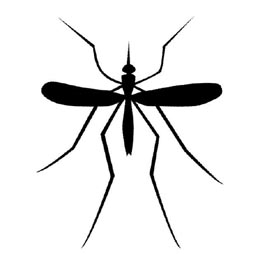
\includegraphics[width=0.4\columnwidth]{pics/mosquito}
	%\caption{}\label{fig:m}
\end{figure}
\newpage

%Udelat titulni stranu!

\section{Popis úlohy}

		Řešená úloha je inspirována článkem Backyard star wars \cite{zadani}. Pohyblivá
		kamera sleduje simulovaného komára, který je představován černým čtvercem na
		bílém pozadí monitoru. Pohyb kamery je možné řídit natočením okolo svislé osy
		(změnou azimutu) a natočením okolo vodorovné osy (změnou elevace). Cílem úlohy
		je řídit kameru tak, aby sledovala pohyb komára a zdokumentovala jeho „sestřel“
		sérií snímků, ve kterých je komár ve středu obrazu z kamery – uprostřed
		„záměrného kříže“.

\section{Rozbor problému}

		Úloha se skládá z několika oblastí, především je zde zastoupena oblast
		počítačového vidění, kdy je nutné sejmout obrázek z kamery, zpracovat ho a
		detekovat v obraze komára. Další oblastí, která je zastoupena, je řízení, celý
		program tvoří zpětnovazební smyčku, pro regulaci je použit PI regulátor. Pro
		lepší funkci je nutné najít a implemtovat vhodný způsob predikce pohybu komára.
		V neposlední řadě je v problému zastoupena robotika, kdy je potřeba pracovat se
		soustavou serv a počítat transformace souřadnic mezi obrazovkou a souřadným
		systémem serv.

\section{Změny specifikace}


		Oproti první etapě nastaly především změny v regulátoru, primitivní P regulátor
		byl rozšířen o integrační složku a obě konstanty byly důkladněji naladěny řadou
		provedených testů. Dále byla v souladu se zadáním druhé etapy vylepšena funkce
		pro určení polohy komára v obraze z kamery tak, aby si správně poradila s případnou
		přítomností okrajů obrazovky ve snímku a kód této funkce byl optimalizován.
		Program byl změněn tak, aby sejmuté obrázky nevykresloval,
		ale pouze je zaznamenával a tím se jeho běh zrychlil. Pro zpětné („offline“) vizuální 
		vyhodnocení úspěšnosti „sestřelu“ byla implemtována funkce \textit{playResults},
		která zobrazí sekvenci zaznamenaných snímků.


\section{Řešení problému}

		Rámec programu je tvořen zpětnovazební regulační smyčkou pro řízení polohy
		kamery. Vstupem regulátoru je nejnovější získaný obrázek z kamery a jeho
		výstupem je nová poloha kamery. Schématicky je to znázorněno na
		obrázku~\ref{fig:ridiciSystem}.  Před samotným výpočtem nové polohy kamery
		je vyhodnocen nově získaný obraz. Postup jeho zpracování je znázorněn na
		obrázku~\ref{fig:zpracovaniObrazu}.  Nejprve je určena poloha komára v obraze
		(funkce \textit{findMosquitoInImage}) v pixelových souřadnicích. Na základě odchylky
		této polohy od středu obrázku potom funkce
		\textit{mosquitoPxPositionToAzimuthAndElevation} počítá odhad úhlů, o které je
		komár vychýlen od optické osy kamery. Pro urychlení celé smyčky jsou data pouze
		logována, nikoliv zobrazována. Uživatel si snadno tato data přehraje offline.

		\begin{figure}[!h]
			\centering
			 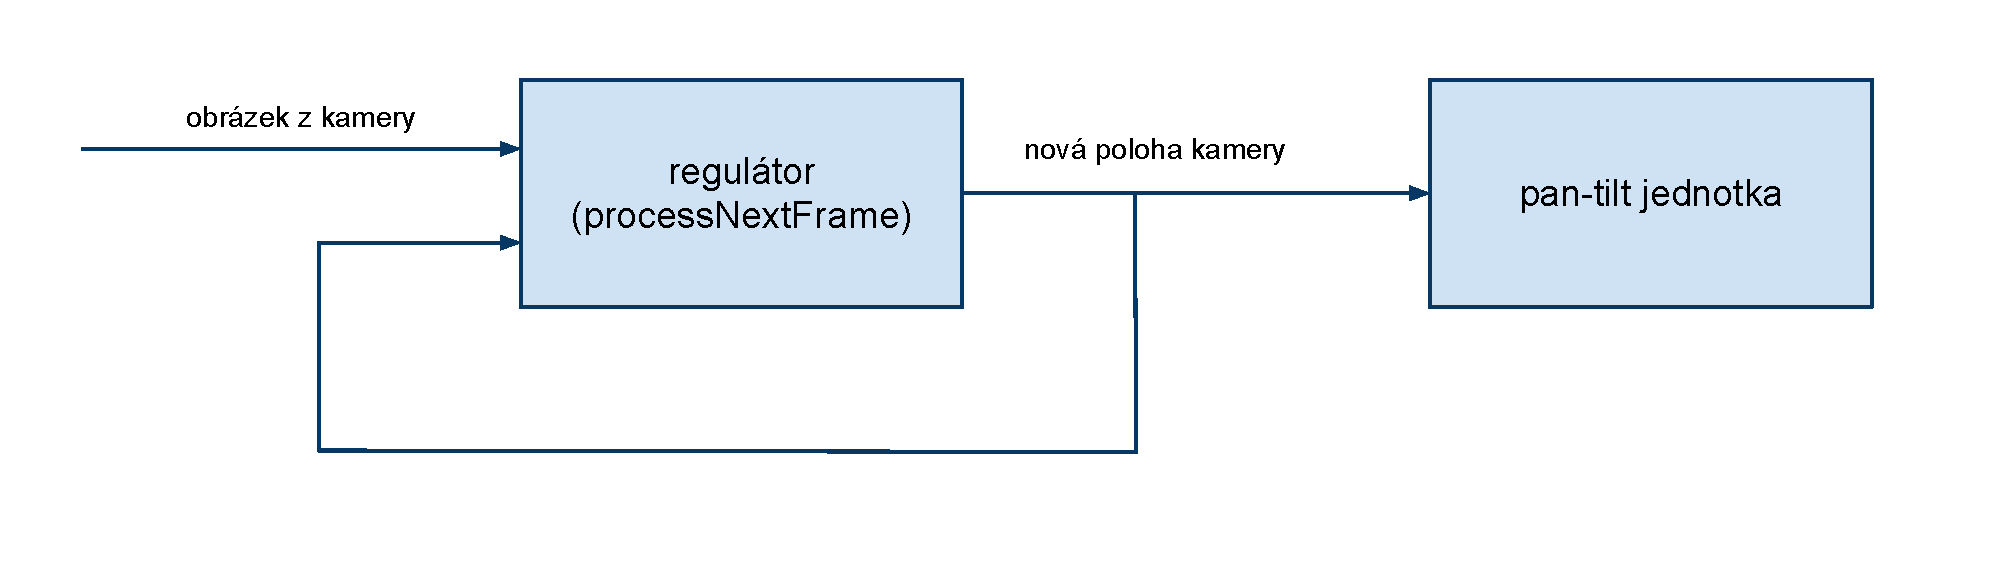
\includegraphics[width=1\columnwidth]{pics/schema_ridiciho_systemu}
			 \caption{Schéma řídícího systému}\label{fig:ridiciSystem}
		\end{figure}


\section{Implementace}

\subsection{Hlavní metody}

		Program se spouští hlavní metodou \textit{startMosquitoHunter}:

		Po spuštění funce se zinicializuje servo mechanismus tak, aby se kamera
		nastavila na střed obrazovky, jedná se o startovní konfiguraci, ve která kamera
		čeká dokud komár nepřilétne do jejího zorného pole. Tento postup je sice
		pasivní, ale experimenty prokázaly, že oproti aktivímu vyhledávání komára na
		počátku programu je časově efektivnější. Aktivním vyhledáváním je myšlen
		algoritmus, kdy kamera sekvenčně snímala pruhy obrazovky a vyhledávala komára.

		Jako další krok se zincializuje kamera a s využitím
		callback funkce se volá \textit{processNextFrame}, která zahrnuje hlavní chod
		programu. Perioda spouštění je nastavena na dvojnásobek snímací frekvence, k regulaci se používá každý druhý obrázek.
		Tato perioda je nastavena jako základní testovací, do třetí etapy bude program časově optimalizován.

		\begin{figure}[!h]
			\centering
			 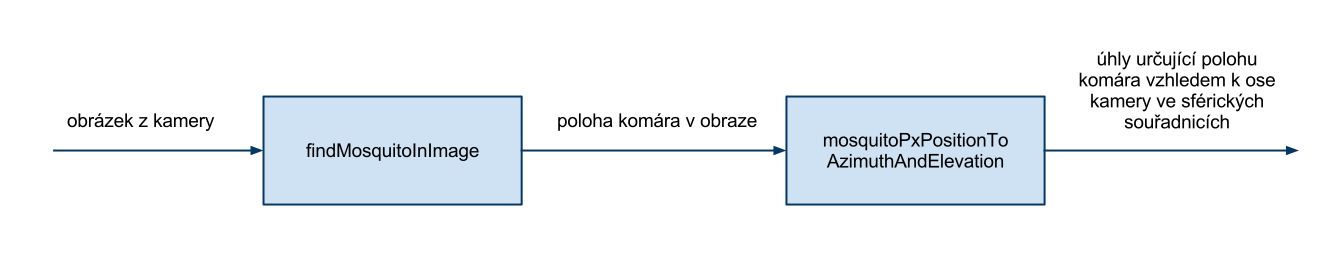
\includegraphics[width=1\columnwidth]{pics/zpracovani_obrazu_z_kamery}
			 \caption{Zpracování obrazu z kamery\label{fig:zpracovaniObrazu}}
		\end{figure}


\vspace{0.5cm}
\textit{processNextFrame}

		Tato funkce pracuje s jedním obrazem získaným z kamery, upraví ho využitím de
		bayerizace. Takto upravený obraz předá funkci \textit{findMosquitoInImage},
		jejíž návratové hodnoty jsou $x, y$ souřadnice středu komára v obraze. Tyto
		hodnoty jsou předány funkci \textit{mosquitoPxPositionToAzimuthAndElevation},
		která vypočte hodnoty azimutu a elevace. 

	        Regulace, tedy výpočet nové polohy kamery $x_{new}, y_{new}$ je řešena jako PI
		regulátor v těle funkce \textit{processNextFrame}. 
	        Vypočte se rozdíl mezi skutečnou a žádanou hodnotou $err$ a do
		proměné $sum_e$ se tato odchylka přičítá, při čemž její počáteční hodnota je
		nulová. Proměné $x, y$ jsou souřadnice aktuální polohy kamery.

		$$x_{new} = x + P\cdot err + I\cdot sum_e$$
		$$y_{new} = y + P\cdot err + I\cdot sum_e$$

		Pozice kamery je saturována na hodnoty, ve
		kterých je očekáván komár, tedy na hodnoty odpovídající kraji monitoru.

		Do třetí etapy regulátor bude vylepšen o naladění $P, I$ složek pro každou osu
		zvlášť a doplnění o antiwind-up. 

		\vspace{0.5cm}
		\textit{findMosquitoInImage}

		K získání polohy komára v obrazu z kamery byl použit jednoduchý algoritmus
		využívající morfologických funkci Matlabovského Image Processing Toolboxu. Jedná
		se o funkce \textit{bwlabel} pro nalezení souvislých oblastí a funkce
		\textit{regionprops} pro určení délky (vlastnost \textit{MajorAxisLength}) a
		plochy (vlastnost \textit{Area}) těchto oblastí.

		%kdyz je to efektivnejsi, proc to nedelame? '' empiricky urcena hodnota? histogram se nelibil? '' jejíchž?

		Komár zobrazovaný na monitoru pracoviště je představován černým čtvercem na
		bílém pozadí. Barevná informace je proto zanedbávána a použit je pouze obrázek
		ve stupních šedi (efektivnější by bylo použít pouze jednu z barevných složek).
		Tento obrázek je následně porovnán s empiricky určeným prahem, tím vznikne binární maska s oblastmi, 
		které vykazují barevnou podobnost s hledaným komárem. 
		%oblasti s jasem
		%menším vykazují barevnou podobnost s hledaným komárem.
	    
		V této masce
		jsou nalezeny souvislé oblasti právě využitím funkce \textit{bwlabel}. Z
		nalezených oblastí je vybrána ta, kterou považujeme za komára. Pro toto
		rozhodnutí jsou použity vlastnosti oblastí \textit{MajorAxisLenght} a
		\textit{Area}. Jsou vyloučeny takové oblasti, jejichž plocha je větší než $3000$
		pixelů nebo jejichž délka je více než $50$ pixelů. Tyto hodnoty byly nastaveny
		na základě maximálních parametrů komára a dostatečné rezervy. Ze zbývajících
		oblastí je vybrána ta, která má největší plochu. Pro tuto oblast je určena
		poloha středu v pixelových souřadnicích a tato infromace je návratová hodnota
		funkce \textit{findMosquitoInImage}.

		% Z barevného obrázku se nejprve vytvoří obrázek šedotónový uložený ve formátu
		% uint8. Po té se naleznou oblasti, ve kterých je podezření na komára na základě
		% znalosti, že komár je tmavý obrazec na světlém pozadí. Tyto oblasti se
		% vyhodnocují na základě histogramu obrázku, hodnoty světlejší než intenzita 200
		% se zahodí. Tato hodnota byla experimentálně určena, s dostatečnou jistotou
		% oblast komára není světlejší, maximální světlost byla pozorována pod hodnotou
		% 100. Ve zbylé části histogramu se vyhodnotí maximum četností. Práh pro detekci
		% komára je stanoven jako dvojnásobek této hodnoty – dostatečné pokrytí rozložení
		% intenzit kolem maxima. 

\vspace{0.5cm}
\textit{mosquitoPxPositionToAzimuthAndElevation}

		V této funkci se přepočtou souřadnice v pixelech obrazu na informaci o azimutu a
		elevaci.

		% konkrétnější popis

\subsection{Pomocné metody}

		\begin{itemize}
				\item \textit{addCrosshairToThePicture} Do středu obrázku vykreslí kříž zadané tloušťky. 
				\item \textit{deBayerize} Provede deBayerizaci obrázku.
				\item \textit{initLoggingVariables} Zinicializují se proměné potřebné pro ukládání dat.
				\item \textit{logData} Ukládá obraz, pozici komára, posun kamer, potřebný čas k běhu a další proměné pro zpětné testování funkcí.
				\item \textit{playResults} Přehraje uložené obrázky s vykresleným záměrným křížem.
				\item \textit{stopMosquitoHunter} Ukončí práci s kamerou a servo mechanismem.
		\end{itemize}

\section{Experimentální výsledky}
		Cílem etapy bylo zoptimalizovat detekci komára v obraze. 
		S využitím Matlabovských funkcí \textit{tic} a \textit{toc} byl měřen čas vykonávání funkce, 
		tento experiment byl třicetkrát zopakován a naměřený čas byl zprůměrován, funkce v průměru trvala $0,08 s$. 
		Minimální perioda s jakou je možné získat obrázky z kamery je $0,067 s$, proto by bylo potřeba běh funkce ještě více zrychlit, bohužel z vyzkoušených algoritmů žádný neodpovídal lépe daným požadavkům. 

		V první etapě byl pro regulaci implementován pouze jednoduchý P regulátor, což mělo za následek, 
		že kamera byla vždy pozadu za skutečnou pozicí komára. Přidáním integrační složky se dosáhlo zlepšení tohoto stavu. 
		Jako další experiment bylo provedeno měření vzdálenosti středu komára od středu obrázku. 
		Toto měření bylo zopakováno 300 krát a průměrná vzdálenost je $14,3 $ pixelů.



\section{Diskuze a Závěr}
		Cíl druhé etapy byl naplněn, čas detekce komára v obraze považujeme za uspokojující, ale pro maximální rychlost smyčky je potřeba výpočet zrychlit. Do třetí etapy bychom rádi prostudovali další literaturu a upravili algoritmus tak, aby běh smyčky byl ještě rychlejší. 

		Dále byl vylepšen regulátor přidáním integrační složky. Do třetí etapy bude regulátor upraven tak, 
		aby komára dokázal bezpečně sledovat i při vyšších rychlostech.
		Za tímto účelem bude smyčka doplněna o predikci pohybu komára. Celý program bude upraven tak, aby efektivně využíval přiděléné prostředky.
		Na řadě experimentů bude otestována funkčnost. 

\bibliographystyle{splncs03}
\bibliography{report}







\end{document}
